%!TEX TS-program = xelatex
%!TEX root = ../../maxwell2018thesis.tex

\chapter{Introduction}\label{chap:intro}
Today, we live in the \emph{Information Age,} an era of human history characterised by the rapid development of technology -- allowing for the creation, transmission and retrieval of large volumes of information. Two key developments that have permitted such an increase in information generation are the electronic computer and the associated technologies that allow for near-instantaneous communication with devices all around the planet, including the \emph{Internet} and~\gls{acr:www}~\citep{berners1994www}.

\begin{figure}[h]
    \centering
    \vspace{5mm}
    \resizebox{1\hsize}{!}{
    
\includegraphics{figures/ch1-earth.pdf}}
    \label{fig:earth_satellites}
    \vspace{-4mm}
\end{figure}

Since the early 1990's, the~\gls{acr:www} has emerged as the dominant means of publishing information online over the Internet, replacing obsolete technologies such as the \emph{Gopher} protocol.\footnote{Gopher was designed primarily with a menu-driven interface in mind (i.e. selecting options from a series of choices). The Gopher ecosystem provided the foundations for the~\gls{acr:http} protocol, which the~\gls{acr:www} today utilises.} As the amount of information available on the~\gls{acr:www} grew, so too did the paradigms that were employed by those wishing to seek information on it.

\emph{Information seekers} would traditionally \emph{surf} the~\gls{acr:www}, starting from a particular domain and navigating through the~\gls{acr:www} via a series of \emph{hyperlinks} within documents. This proved practical, as portal websites typically presented categorised lists of websites, much like a telephone directory. However, as the volume of content available on the~\gls{acr:www} grew ever larger, this approach became impractical. Information seekers began to use \emph{search engines} -- referred to as \emph{retrieval systems} in this thesis -- as a means of \blueboxbold{searching} the ever increasing universe of documents available at their disposal (refer to Figure~\ref{fig:ch1-surfing}).\footnote{\cite{mcbryan1994taming_tools} considered a retrieval system as a means of \emph{taming} the considerable number of documents online.}

This is not to say that surfing no longer occurs. Information seekers today will typically use a retrieval system to find a particular domain, then begin surfing within said domain to find the information that they seek, if such information is not found immediately by the retrieval system. However, with the large volume of information now online, retrieval systems are the most effective way to locate information. Helping \emph{searchers} realise this is seen as the \emph{raison d'\^{e}tre} of the study of~\gls{acr:ir}.

\begin{quote}
    \emph{``...but perhaps the key technology that took the web from a useful supplement of current information practice to become the default communication medium is search.''}
    \attrib{\cite{wilson2010keyword_search}}
\end{quote}

Contemporary commercial retrieval systems such as \emph{Google} and \emph{Bing} are considered to offer an effective means of finding the proverbial needle in the haystack~\citep{wilson2010keyword_search}, where near perfect accuracy is regularly attained for popular \emph{queries}~\citep{vaughan2004new_measurements}. These retrieval systems, along with the many others in existence today under a variety of contexts\footnote{Google and Bing may be the most popular retrieval systems for \emph{general web queries,} but other contexts, for example, can include patent search, enterprise search and multimedia search.}, are the product of the collective work undertaken in the field of~\gls{acr:ir}, as we discuss in more detail in Chapter~\ref{chap:ir_background}.

\begin{figure}[t!]
    \centering
    \resizebox{1\hsize}{!}{
    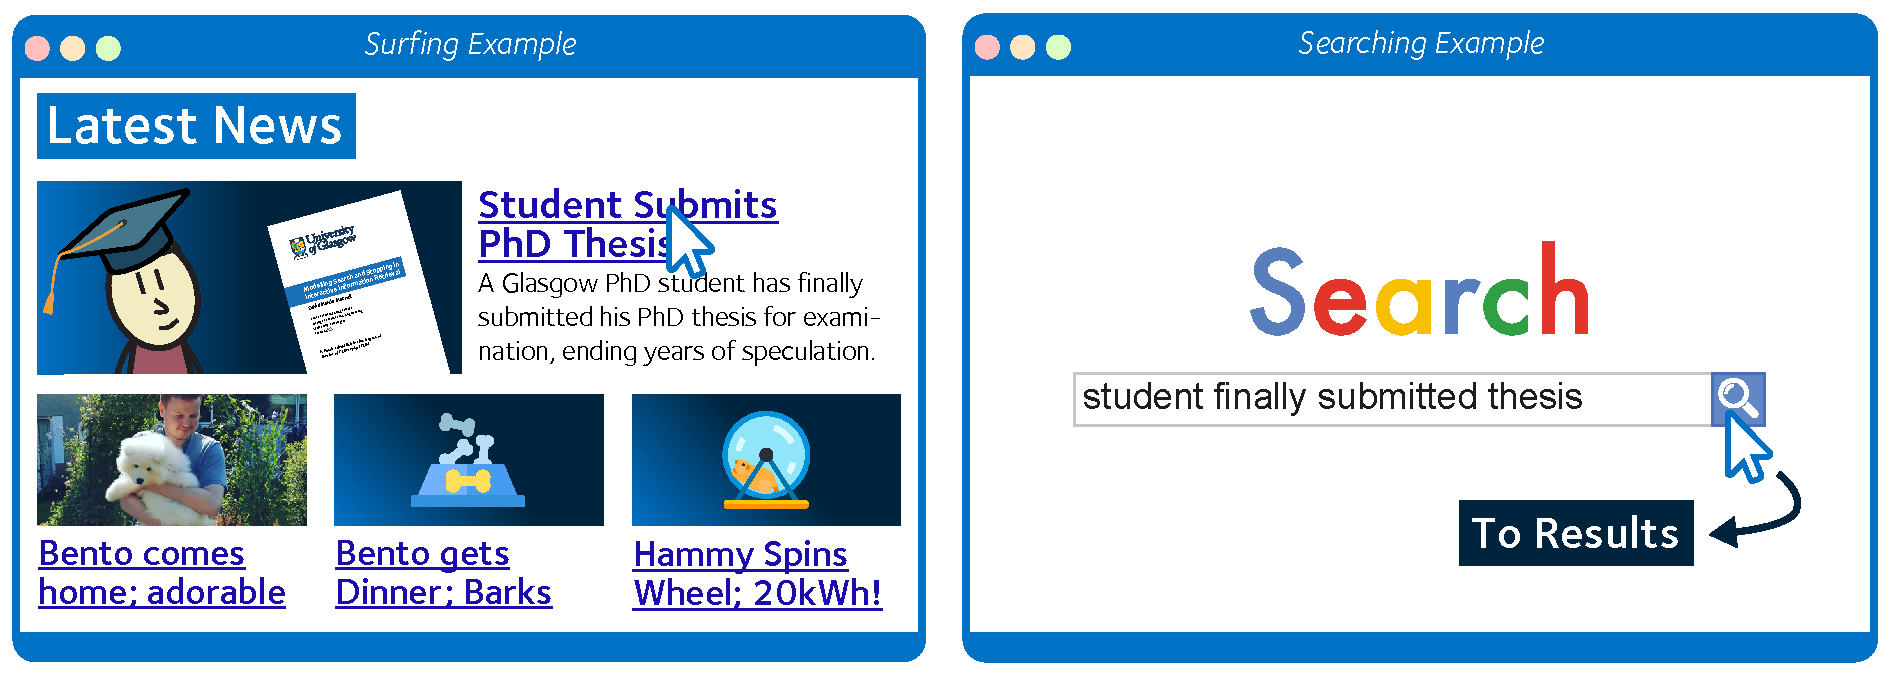
\includegraphics{figures/ch1-surfing.pdf}}
    \caption[Surfing vs. searching: illustrations of the two paradigms]{The paradigms of surfing and searching. On the left, a seeker will navigate through a series of documents via~\glspl{glos:hyperlink} (perhaps without a specific \emph{information need} in mind), while a searcher (right) will issue a \emph{query} articulating their information need, relying on a \emph{retrieval system} to retrieve a series of documents that are judged to be of use to the seeker.}
    \label{fig:ch1-surfing}
\end{figure}

The field of~\gls{acr:ir} aims to make it easier for searchers to satisfy their underlying \emph{information need.} A searcher will develop an information need from a perceived problem -- either from a knowledge gap, an internal inconsistency, or a conflict of evidence. This state has been referred to as the \emph{Anomalous State of Knowledge (ASK)}~\citep{belkin1980ask}. A searcher, once they have realised this information need, will formulate a \emph{query} -- an expression of what they are looking to seek~\citep{borlund2003iir_model}, typically consisting of a number of different terms. This query is then submitted to the retrieval system, before a potentially relevant set of documents -- as judged by the retrieval system -- are returned to the searcher. From this set of documents, the searcher can then begin the process of examining them for relevance.

A number of complex interactions take place between an individual seeking information and the retrieval system being utilised~\citep{ingwersen2005theturn}. This interactive process, where the searcher engages in dialogue with the retrieval system, is considered the study of~\gls{acr:iir}~\citep{borlund2003iir_model}. One of the fundamental aspects of~\gls{acr:iir} is that of \blueboxbold{stopping} -- where, for example, a searcher must decide when to stop examining the list of results returned to him or her.

Examining stopping behaviour is one of the many different interaction aspects that have been examined to help us better understand a searcher's behaviours, and potentially assist in making the search process a more seamless experience for said searchers. As we discuss in the next section, much of the research in both~\gls{acr:ir} and~\gls{acr:iir} has been limited in terms of examining these interactions. Subsequently, these limitations provide motivation for the work detailed in this thesis.

\section{Motivation and Context}
Central to much of the work undertaken in the field of~\gls{acr:ir} is the \emph{Cranfield paradigm,} a term denoting a standardised approach of~\gls{acr:ir} evaluation~\citep{aslib1966factors}. Primarily credited to Cyril Cleverdon at Cranfield University\footnote{Cranfield University is located at Cranfield, Bedfordshire, England. It is unique in that it has a semi-operational airport, given its heritage with aeronautics research.}, the paradigm revolves around the notion of standardised \emph{test collections} -- standardised corpora of documents that can be used by different researchers, providing an uniform foundation for~\gls{acr:ir} experimentation.

While the basic principles of the Cranfield paradigm have remained in place since it was established in the 1960's, aspects of the approach have evolved over the years to cater for the ever increasing complexity of the tasks trialled~\citep{harman2010cranfield}. The approach is widely used in evaluation forums, such as \emph{NTCIR (NII Testbeds and Community for Information access Research)} and \emph{CLEF (Conference and Labs of the Evaluation Forum).} However, one of the best known evaluation forums following the paradigm is the~\gls{acr:nist} sponsored~\gls{acr:trec}~\citep{harman1993trec1}. Indeed, the work reported in this thesis extensively utilised material generated as part of~\gls{acr:trec} efforts, provided as part of different \emph{\gls{acr:trec} Tracks} over a number years.

With the Cranfield paradigm, significant advances have been possible regarding the evaluation of~\gls{acr:ir} systems. However, the approach can be argued to be somewhat limited from the context of~\gls{acr:iir} as it does not consider the interactions that take place between a searcher and a retrieval system~\citep{borlund2000evaluation_iir, ingwersen2005theturn}. In other words, the paradigm broadly fails to consider the complexities of the~\gls{acr:iir} process. As an example of such a complexity, searchers could issue multiple queries during the course of a search session. Subsequently, they would adapt their interactions based upon the perceived quality of presented ranked result lists~\citep{moffat2013users_versus_models}.

A key example of such behaviour adaption is the searcher's stopping behaviour. For example, a poor set of results may mean that searchers would stop examining results comparatively early than a set of results perceived to be of good quality. Searchers also often stop once they feel that they have found sufficient information to satisfy their information need~\citep{zach2005enough_is_enough}. Indeed, selecting good terms to use within a query is difficult yet important~\citep{efthimiadis2000query_expansion}. The initial query posed in a search session often acts as an entry to the search system, following by phases of browsing and query reformulations~\citep{marchionini1993information_seeking}. Searchers also will typically abide by the \emph{principle of least effort,} whereby they strive to minimise the expected rate of work expenditure over time~\citep{zipf1949behaviour}.

The experimentation paradigms that have evolved from Cranfield -- such as that employed in~\gls{acr:trec} experimentation -- make a series of different assumptions that are largely at odds with how searchers interact with retrieval systems. Namely, these assumptions state that a searcher will:

\begin{itemize}
    \item{issue a \emph{single query} over the course of a search session;}
    \item{\emph{examine documents to a certain depth} (typically $1,000$ in~\gls{acr:trec} experimentation); and}
    \item{\emph{consider all documents to be relevant} to the given information need.}
\end{itemize}

While providing a simple platform for performing retrieval system evaluation, such assumptions are unrealistic. Herein lies a fundamental disconnect between the studies of~\gls{acr:ir} and~\gls{acr:iir} -- the na\"{i}ve assumptions made of searchers within~\gls{acr:ir} experimentation listed above do not hold when considering the complex interactions that actually take place during the~\gls{acr:iir} process~\citep{ingwersen2005theturn}. In order to address the fundamental disconnect between the two fields, we need to create \blueboxbold{more realistic searcher models} that better articulate what real-world searchers actually do. Work has been undertaken in the field of~\gls{acr:iir} to address this, examining searcher behaviours under a number of different phenomena, including (but not limited to) the following:

\begin{itemize}
    \item{\emph{query formulation and suggestions}~\citep{azzopardi2009query_side, azzopardi2007languages, baskaya2013behavioural_factors, carterette2015test_collections, jordan2006cqg, keskustalo2009querying, verberne2015personalised_queries};}
    \item{\emph{browsing behaviours}~\citep{carterette2015test_collections, chuklin2015click_models, guo2009click_chain, pakkonen2015behavioural_dimensions, smucker2011user_strategies};}
    \item{the influence of \emph{costs and time}~\citep{azzopardi2011economics, baskaya2013behavioural_factors}; and}
    \item{\emph{performance over search sessions}~\citep{luo2014winwin, luo2015pomdp}.}
\end{itemize}

When considering how we model searcher interactions, a further (and particularly important) phenomenon not listed above is that of a \blueboxbold{searcher's stopping behaviour}. Indeed, given its title, this is what we consider in this thesis -- \emph{how can we make improvements to searcher models when considering stopping behaviours?} This phenomenon has been largely overlooked in the literature~\citep{maxwell2015stopping_strategies}, yet is in contemporary research seeing an increasing amount of time dedicated to its examination. In the following subsection, we provide an argument as to why examining this phenomenon is important, and what benefits we can derive from its examination.

\subsection{Considering Stopping Behaviours}
Knowing when to stop is a fundamental aspect of animal -- and by definition, human -- thinking and behaviour. There must come a time when an animal must stop what it is doing. In the natural world for example, a honeybee, when \emph{foraging} for pollen, will eventually make a decision to stop collecting pollen on the flowerhead it finds itself on and fly away to another flowerhead. The honeybee is in essence attempting to maximise the amount of \emph{gain} (pollen) she accumulates over time on each \emph{patch} (flowerhead) that is visited.

\begin{figure}[t!]
    \centering
    \resizebox{1\hsize}{!}{
    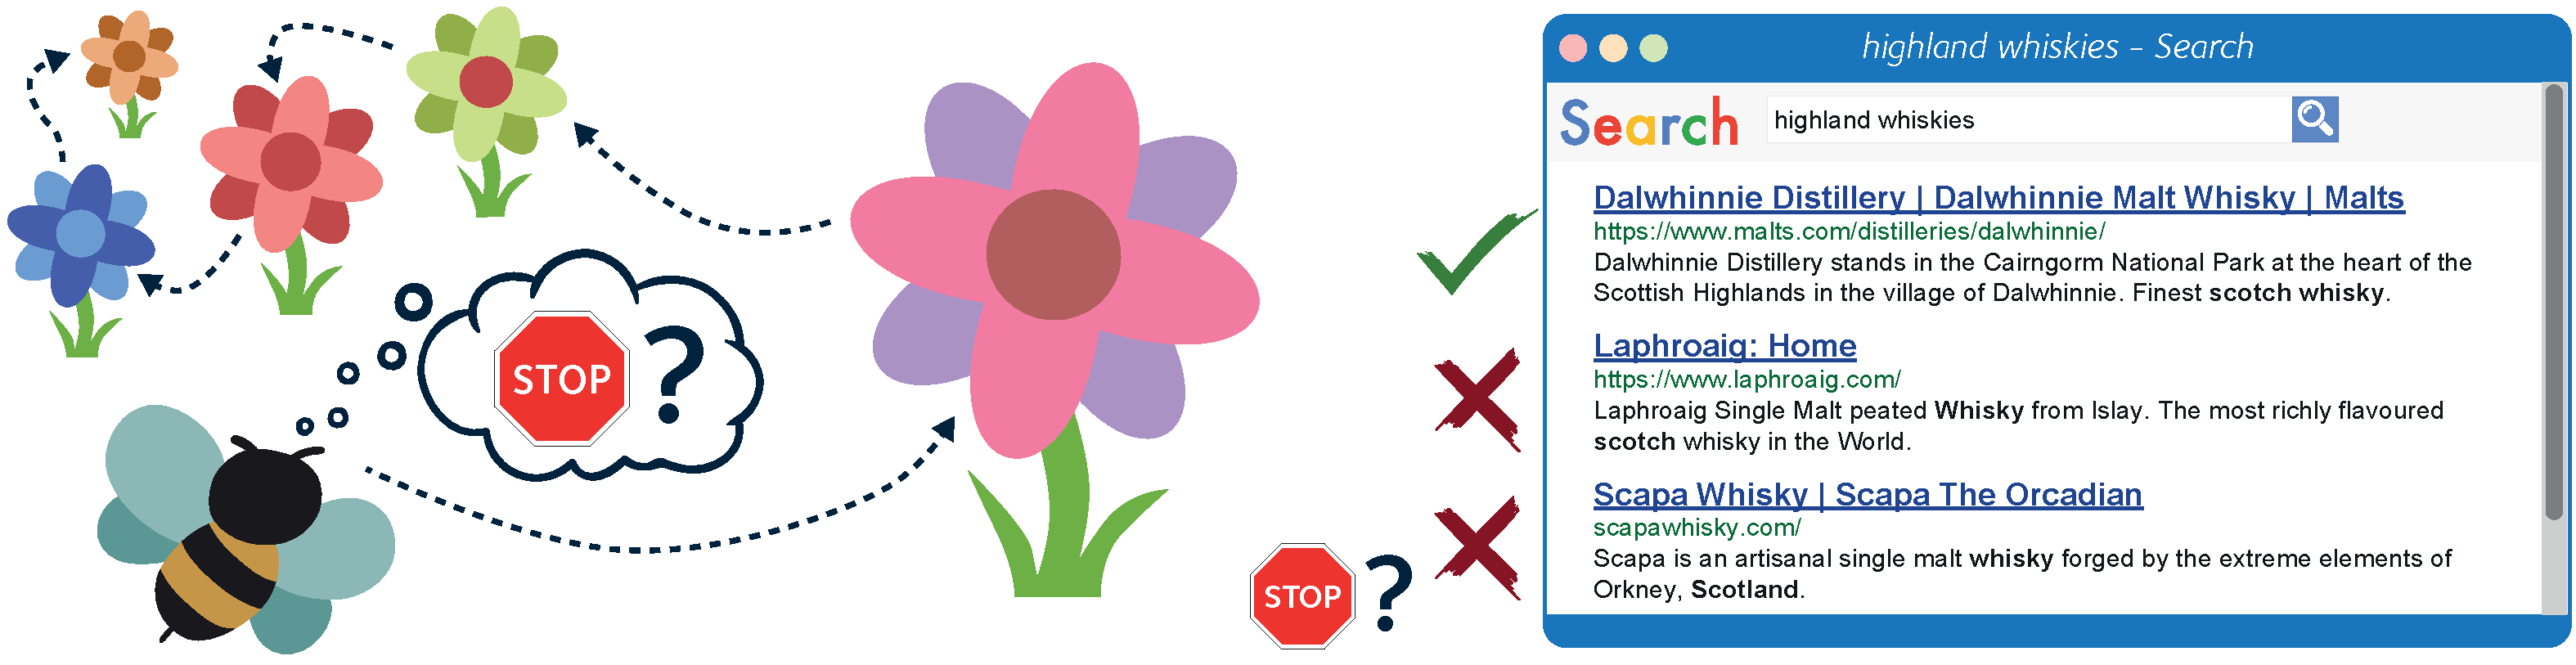
\includegraphics{figures/ch1-stopping.pdf}}
    \caption[Animal and searcher stopping examples]{Examples of stopping. On the left, when will the bee move from one flowerhead to the next? On the right, under the context of information seeking, how far down a list of ranked results will a searcher go before he or she decides to stop examining content? In the example above, \searchlogo~has failed to return a comprehensive list of highland single malt whiskies~
\includegraphics[height=\fontcharht\font`\d]{figures/ch0-saltire.pdf}. Will the searcher become frustrated with this, and stop examining results comparatively early?}
    \label{fig:ch1-stopping}
\end{figure}

If we consider stopping from an information seeking context, there are many different examples we can use to demonstrate why this behaviour is of great importance. For example, a searcher may decide to stop searching for information when the documents presented show a large volume of non-relevant material, frustrating said searcher~\citep{cooper1973retrieval_effectiveness_ii} -- perhaps because the retrieval system failed to gauge the searcher's \emph{query intent}~\citep{ashkan2009classifying}, as demonstrated in Figure~\ref{fig:ch1-stopping}. Searchers could also stop examining content after they have become satisfied with the information found previously in a search session~\citep{cooper1973retrieval_effectiveness, gibb1958number_rule, simon1955satiation}, or if they feel that the information being presented is too similar to what has been found earlier~\citep{nickles1995judgment}.

Obviously, a number of different \emph{external factors} influence the decision of when one should stop; such as finding a flowerhead with no pollen, or time pressures when searching for information. However,~\cite{nickles1995judgment} argues that \emph{knowing when to stop} is largely determined by a series of \emph{internally defined stopping criteria} that the decision maker employs, just like the examples defined above. This internal construct makes stopping a phenomenon that is difficult to model in an effective way.

Given that internal factors are a major drive in determining when to stop, studies have largely been unable to quantify \emph{why} searchers stop, other than what they find during the search process gives them the feeling that it is \emph{``good enough''} to satisfy their information need~\citep{zach2005enough_is_enough}. Like the stopping examples defined above, researchers have attempted to create a series of reasoning- and judgement-based \blueboxbold{stopping heuristics} that attempt to formally define when a searcher should stop. It is these stopping heuristics that we will primarily consider in this thesis. These heuristics can then be integrated within a wider searcher model, allowing us to determine whether they improve or worsen approximations of actual searcher stopping behaviours. The searcher model can incorporate stopping behaviours at a variety of different \blueboxbold{stopping decision points} -- such as at an individual result summary level \emph{(how far down this list of ranked results should I go?),} or at a session level \emph{(how many queries should I issue before stopping my search session?).}

Examining stopping behaviours during search is important because it considers the judgements of a searcher as part of their interactions. For example, it would be prudent of a searcher examining a ranked list of results that are mostly non-relevant to stop early, thus saving time and effort. In other words, a searcher employing a sensible stopping heuristic is therefore \emph{more efficient.} Stopping behaviour is also implicitly or explicitly encoded within a variety of different~\gls{acr:ir} and~\gls{acr:iir} measures. Obtaining a better understanding of when searchers stop means that we can encode this information within measures of search (improving their credibility), and provides an evidence-based approach to mapping these measures with what actually takes place in reality.

\section{High-Level Research Questions}\label{sec:intro:rqs}
Having set out the problem space above, we can now begin to formulate the four high-level research questions that the work in this thesis addresses, denoted as \darkblueboxbold{HL-RQx}. Our first research question considers the concept of modelling searchers, and how, with an emphasis on examining stopping decision points, we can improve current models to better reflect actual searcher behaviours -- in particular, their stopping behaviour.

\begin{itemize}
    \item{\darkblueboxbold{HL-RQ1} How can we improve searcher models to incorporate different stopping decision points?}
\end{itemize}

As previously stated, being able to improve upon the current searcher models from the perspective of stopping should allow those subscribing to such a model to become more efficient as to how they search. Closely related to this advancement in modelling this process is the consideration of the various stopping heuristics.

\begin{itemize}
    \item{\darkblueboxbold{HL-RQ2} Given the stopping heuristics defined in the literature, how can we encode these heuristics into a series of \emph{operationalised,} programmable \blueboxbold{stopping strategies} that can be subsequently incorporated into the searcher model and be evaluated?}
\end{itemize}

Stopping heuristics that we detail later in Section~\ref{sec:stopping_background:heuristics} are high-level in nature, and do not provide an explanation as to how they can be operationalised within a wider system. The challenge that must be addressed in order to answer this second high-level research question will therefore be how we can operationalise such stopping heuristics as a series of programmable stopping strategies.

With a more realistic searcher model from \darkblueboxbold{HL-RQ1} and a series of stopping strategies defined by addressing \darkblueboxbold{HL-RQ2}, how well does this combination perform?

\begin{itemize}
    \item{\darkblueboxbold{HL-RQ3a} Given the aforementioned operationalised stopping strategies, how well does each one perform?}
    \item{\darkblueboxbold{HL-RQ3b} How closely do the operationalised stopping strategies compare to the actual stopping behaviours of real-world searchers?}
\end{itemize}

These questions are of course of a very broad nature, and it is simply not possible to evaluate them in every conceivable search context. As such, we will examine several contexts that are likely to impact upon searcher stopping behaviours. Specifically, we will examine topical \emph{interactive search} in the domain of news, where we will consider various conditions: search goals and task types; search durations; and result summary length. In the following section, we expand upon these conditions to provide a concrete set of thesis contributions.

\section{Thesis Contributions}\label{sec:intro:contribs}
This thesis presents four major contributions. Listed below, we consider primary contributions from conceptual, theoretical, methodological and empirical standpoints.

\noindent
\dualbluebox{Conceptual}{Complex Searcher Model} Our first contribution is a new searcher model. Taking current searcher models, we propose an updated, high-level model of the search process called the~\gls{acr:csm}. This provides us with a solution for addressing \darkblueboxbold{HL-RQ1}. Outlined in Chapter~\ref{chap:csm} (page~\pageref{chap:csm}), the conceptual~\gls{acr:csm} outlines a series of different activities and decision points that searchers undertake throughout the search process, and establishes a flow of interaction based upon established models. Within the~\gls{acr:csm} are a number of different innovations, the central innovation being a new stopping decision point. For example, this improvement allows us to ascertain a better understanding of the search process, and the complex interactions between a searcher and retrieval system that occur. Being a conceptual model, we can take the~\gls{acr:csm} and instantiate it in a number of different ways. The stopping strategies that we consider in this thesis for example provide a means for instantiating stopping decision points within the~\gls{acr:csm}.

\noindent
\dualbluebox{Theoretical}{Stopping Strategies} As previously discussed, there are a range of different stopping heuristics that have been defined in the literature that provide an explanation for when searchers should stop examining content. The second major contribution of this thesis is the development of twelve operationalised, programmable stopping strategies that may be subsequently implemented as a stopping decision point of the~\gls{acr:csm}, as defined above. These twelve strategies encode a total of eight different stopping heuristics and~\gls{acr:ir} measures. The operationalised stopping strategies provide a solution to \darkblueboxbold{HL-RQ2}.

\noindent
\blueboxbold{Methodological} The proposed~\gls{acr:csm} and the twelve stopping strategies that we operationalise need to be evaluated, such that we can then subsequently address the two remaining high-level research questions, \darkblueboxbold{HL-RQ3a} and \darkblueboxbold{HL-RQ3b}. To do this, a general methodology outlines approaches undertaken for user studies. \blueboxbold{Simulation} is used to determine how the different stopping strategies perform over each of the different search contexts trialled, and how the stopping strategies compares to actual searcher behaviour.

\noindent
\dualbluebox{Empirical}{Varying Result Summary Length} We report on a study where the length of individual result summaries presented to searchers are varied to determine what impact that this has on searcher stopping behaviour. As we modify the length of result summaries, we also argue that we influence the overall quality of result summaries. We then perform a simulated analysis examining each of the stopping strategies, determining what strategies perform best and offer the closest approximations to real-world stopping behaviours.

\noindent
\dualbluebox{Empirical}{Varying Goals and Tasks} We report on an additional user study, examining the impact of stopping behaviour when the search task and goals are changed. For this, we consider topical \emph{ad-hoc retrieval}\footnote{The ad-hoc search task is explained in detail in Section~\ref{sec:ir_background:paradigms:trec} -- it is one of many different types of search task that can be performed by searchers.}\emph{,} along with a diversified search task, changing the overall goal of what searchers are looking to find. This is then complemented by a further simulated analysis, examining the individual stopping strategies like above.

\dualbluebox{Empirical}{New Stopping Decision Point} The final empirical contribution complements the conceptual contribution of this thesis, addressing \darkblueboxbold{HL-RQ1}. We perform a further simulated analysis, examining how well the new stopping decision point, when incorporated within the~\gls{acr:csm}, performs -- and whether it offers better approximations to actual searcher stopping behaviours.

\section{Thesis Statement}
Given all of the above, the major claim of this thesis is that by considering a searcher's stopping behaviour, we can develop more credible and realistic models of the search process. These models can then be used as a tool for improving our understanding of the complex interactions that take place while searching, and can potentially aid in the development of more intuitive and user friendly search interfaces that better facilitate searchers in satisfying their underlying information needs.

Moreover, this thesis demonstrates how such stopping behaviours vary under different search contexts, and how the updated searcher model, or~\gls{acr:csm}, is able to effectively model these changes. Specifically, by examining a range of different stopping strategies, the empirical work in this thesis demonstrates what approaches work better under what contexts, and discusses why this may be the case.

% Given all of the above, the major claim of this thesis is that the work presented a deeper understanding of the stopping behaviours exhibited by searchers.
%
% In particular, this thesis explores in detail the various stopping heuristics that have been proposed in the literature, operationalises them as a series of stopping strategies, and empirically evaluates them in terms of their performance and approximations to actual searcher stopping behaviour. A more accurate conceptualisation of the overall search process is also presented in this thesis. By including an additional stopping decision point that we know improves the overall performance and approximations to real-world searchers, we can produce more realistic simulations of interaction.

\section{Origins of the Material}
Material presented in this thesis has appeared in several conference papers and journals throughout the duration of the author's PhD programme, from October 2013 to September 2018. All are listed in the front matter of this thesis in chronological order. In this section, we provide narrative, explaining how the developments in the listed publications led to the contributions of this thesis. Work can be considered over three main strands:

\begin{itemize}
    \item{the development of the conceptual and theoretical contributions to this work;}
    \item{the development of the \simiir~framework; and}
    \item{a series of empirical studies.}
\end{itemize}

\noindent
\blueboxbold{Conceptual and Theoretical}
Work on the~\glsfirst{acr:csm} has been undertaken over a number of years. A number of iterations of the~\gls{acr:csm} were presented in various publications. However, in order to simplify the work reported in this thesis, we consider only the latest iteration. The first iteration of the~\gls{acr:csm} -- essentially analogous to prior models of search outlined in Sections~\ref{sec:ir_background:paradigms:trec:model} and~\ref{sec:ir_background:user:models} -- was used in simulated analyses, as reported in two publications.

\begin{itemize}
    \item{\bibentry{maxwell2015initial_stopping}}
    \item{\bibentry{maxwell2015stopping_strategies}}
\end{itemize}

These publications are notable for also including a number of operationalised stopping strategies, providing the foundations for the second major contribution of this thesis. The stopping strategies defined in these publications were used in subsequent publications. Further developments to the~\gls{acr:csm} were found in a subsequent publication which experimented with the notion of \emph{intelligent search agents}.

\begin{itemize}
    \item{\bibentry{maxwell2016agents}}
\end{itemize}

The final development of the~\gls{acr:csm} led to the inclusion of a third stopping decision point, complete with a large-scale simulated analysis. This led to the finding that the inclusion of a new stopping decision point within the~\gls{acr:csm} provided improvements in overall search performance, and the approximations of actual searcher stopping behaviours.

\begin{itemize}
    \item{\bibentry{maxwell2018serp}}
\end{itemize}

\noindent
\blueboxbold{SimIIR Framework}
One of the major pieces of scientific apparatus utilised throughout all of the aforementioned studies is the \simiir~framework, touched upon in Section~\ref{sec:intro:contribs}. While we do not explicitly discuss the framework in great depth in this thesis, but rather focus on how we implemented the different components, conducting the simulated analyses would not have been possible without it. A publication demonstrating the framework and the various components that could be instantiated has been published.

\begin{itemize}
    \item{\bibentry{maxwell2016simiir}}
\end{itemize}

\noindent
\blueboxbold{Empirical Studies}
The general methodology that we employ for the third major contribution of this thesis has been introduced and refined in the publications listed previously. In addition to this, a basic description of the methodology is provided in a Doctoral Consortium paper that the author presented at the first \emph{ACM Conference on Human Information Interaction and Retrieval (CHIIR)} in Chapel Hill, NC, USA.

\begin{itemize}
    \item{\bibentry{maxwell2016dc}}
\end{itemize}

The results of two user studies have also been published, and are of direct relevance to the work detailed later in this thesis.

\begin{itemize}
    \item{\bibentry{maxwell2017snippets}}
    \item{\todo{\emph{A journal article is currently out for review; hopefully it will be accepted...}}}
\end{itemize}

These studies provide the grounding for simulated analyses that we also consider later in this thesis. The data extracted from these user studies provides credibility to our simulations, through the extraction of aspects such as interaction costs and probabilities.

\section{Thesis Outline}
This section provides a brief summary of the remaining chapters of the thesis. Split into four parts, the chapters are summarised below.

\noindent
\darkblueboxbold{Part I}
The remainder of Part I concerns prior work that has been undertaken in the fields of~\gls{acr:ir} and~\gls{acr:iir}. Two chapters outline the basics of~\gls{acr:ir} and~\gls{acr:iir}, before we begin to examine prior work that considers search and stopping.

\begin{itemize}
    \item[]{\blueboxbold{Chapter 2}} Beginning on page~\pageref{chap:ir_background}, this chapter provides an overview of the key concepts of the fields of~\gls{acr:ir} and~\gls{acr:iir}. In particular, we focus on basic~\gls{acr:ir} concepts, such as the indexing and retrieval processes (including retrieval models). We then move towards a more user-centric examination of various evaluation measures that are commonly deployed in~\gls{acr:iir} research. In particular, we consider a number of different searcher models that have been previously defined in the literature.
    
    \item[]{\blueboxbold{Chapter 3}} We then consider work that has been undertaken in relation to stopping behaviours. In this chapter, we begin by describing various stopping heuristics defined in the literature. We examine previous user studies that have examined searcher stopping behaviours, and then consider key theoretical models of search that provide explanations for when individuals stop.
\end{itemize}

\noindent
\darkblueboxbold{Part II} Beginning on page~\pageref{part:stopping}, Part II presents the conceptual and theoretical contributions of this thesis, including a discussion of the~\gls{acr:csm}. In this part of the thesis, we also provide an outline of the general methodology that is used in Part III.

\begin{itemize}
    \item[]{\blueboxbold{Chapter 4} This chapter introduces the~\gls{acr:csm}, discussing the advances that the conceptual model provides over the contemporary searcher models. We discuss the key stopping decision points provided by the~\gls{acr:csm} that are central to this thesis, before discussing the assumptions of the model. This partly addresses \darkblueboxbold{HL-RQ1} -- evaluation of the model is also required, and discussed in Chapter~\ref{chap:serp}.}
    
    \item[]{\blueboxbold{Chapter 5} In this chapter, we introduce and discuss the various stopping strategies that we operationalise as part of the contributions of this thesis, thus addressing \darkblueboxbold{HL-RQ2}. Each of the different stopping strategies, complete with examples, are discussed in depth. The chosen stopping strategies are linked back to their source stopping heuristics, which are detailed in Chapter~\ref{chap:stopping_background}.}
    
    \item[]{\blueboxbold{Chapter 6} The third chapter of this part outlines our general methodology, detailing the high-level structure of the scientific method used in the empirical work discussed in Part III. We also provide a discussion of common approaches that we used across all subsequent chapters. This methodology allowed us to address all four of our overarching research questions.}
\end{itemize}

\noindent
\darkblueboxbold{Part III}
The third part of this thesis considers the empirical contributions that have been obtained from our studies. In this part, we discuss the user studies that were undertaken, as well as a number of simulated analyses that allow us to address research questions \darkblueboxbold{HL-RQ3a} and \darkblueboxbold{HL-RQ3b}.

\begin{itemize}
    \item[]{\blueboxbold{Chapter 7} The first empirical chapter considers how stopping behaviours vary when the length (and thus quality) of snippets is varied. We provide a discussion of a user study that examined this phenomenon, before summarising the findings of simulated analyses that were conducted in order to determine what stopping strategies offered the best performance and approximations of real-world searchers under this context.}
    
    \item[]{\blueboxbold{Chapter 8} In this chapter, we examine how a searcher's stopping behaviour varies when subjected to the remaining variations that were discussed in Section~\ref{sec:intro:contribs}.}
    
    \item[]{\blueboxbold{Chapter 9} The final chapter wherein novel findings are presented considers the new stopping decision point that is provided by the~\gls{acr:csm}. We empirically test the~\gls{acr:csm}, allowing us to determine whether the inclusion of the new stopping decision point discussed in Chapter~\ref{chap:csm} provides improvements in overall performance and approximations of actual searcher stopping behaviours. As such, this chapter provides sufficient evidence, in conjunction with Chapter~\ref{chap:csm}, to address \darkblueboxbold{HL-RQ1}. We utilise data from user studies discussed in prior chapters to ground the simulations.}
\end{itemize}

\noindent
\darkblueboxbold{Part IV} The final part of this thesis consists of a solitary chapter, \blueboxbold{Chapter 10}. The concluding chapter of this thesis provides a summary of the work that was undertaken, and the results obtained. We then discuss what the results mean in terms of directions for future work.